\section{Methods}\label{sec:Methods}
\subsection{Physics Model Algorithm}
In literature, various MRS physics models have been proposed to simulate brain spectra. They begin with simulated basis functions that are assumed to have been simulated using appropriate pulse sequence parameters for the scenario of interest. These metabolite basis functions are then modulated by scaling factors that indicate their underlying concentrations. Most models then apply a simple Lorentzian lineshape.\cite{Hatami, Das2018a, Das2018} Phase offsets\cite{Das2018,Iqbal2018a} and frequency shifts\cite{Hatami} can optionally be applied. Finally, some type of broad baseline is typically added. These models are simple and do not capture the full complexity of clinical data. Additionally, they often include non-public components such as baselines, macromolecules, and lipid signals that are extracted from private datasets.

To maximize generalizability and usefulness, the data simulator should comprehensively model known spectral components, which were identified through a review of state-of-the-art fitting techniques and currently available fitting algorithms. These spectral components allow the model to account for a large variety of scenarios and artifacts. The physics model proposed in this work is described by the following set of equations:
\begin{subequations}
\begin{equation}
\begin{split}
    f(t)& = \\&\sum_{n}^{N} \underbrace{M_n* basisfcn_n}_{amplitude\ scaling} 
    \underbrace{e^{-d_nt -g_nt^2}_{} }_{lineshape} 
    \underbrace{e^{-i\Delta f_nt}_{}}_{fshift}
    \underbrace{ e^{i(\phi_0 + \phi_1)}_{} }_{phase}
    \underbrace{e^{-iA_0*e^{-t/{{tc}_0}}t*2\pi}_{}}_{eddyCurrents}  * \underbrace{ \sum_{r=1}^R e^{-i\Delta\omega_r t} }_{B_0\ inhomog.}  + 
    \mathcal{H}\left (
    \underbrace{\mathcal{N}\left (0,snr_0, l \right )_{}}_{noise} + baseline + resH_2O \right )
\end{split}
\label{eqn:PM:step1}
\end{equation} \vspace{0.1em}

\begin{equation}
    f(t) = \mathcal{C}{oil}_0^C
    \left ( f(t) { ,\ }\underbrace{\overbrace{{snr_c}_{}}^{noise},\overbrace{sens_c}^{sensitivity}, \overbrace{\Delta f_c, \Delta\phi_c}^{drifts}}_{coil\ artifacts} \right ) \label{eqn:PM:step2} 
\end{equation} \vspace{0.1em}

\begin{equation}
    F(\omega) = \mathcal{F}\left ( zeroFill \left ( f(t) *  \underbrace{e^{-t*T_L}}_{apodize} \right ), len \right )  \label{eqn:PM:step3}
\end{equation} \vspace{0.1em}

\end{subequations}
where $N$ is the whole set of metabolites being modeled, $M_n$ is the scaling factor for metabolite $n$, the Lorentzian variable $d_n$ and the Gaussian variable $g_n$ combine to define a Voigt lineshape, $t$ is time, and $\Delta f_n$ is the metabolite-specific frequency shift. Global zero- and first-order phase offsets are added using $\phi_0$ and $\phi_1$ while eddy current effects are described using two variables as a function of time $t$: the amplitude, $A_0$, and the time constant, $tc_0$. In lieu of the Gaussian term, imperfect shimming and severe lineshape distortions associated with large susceptibility effects can be applied using $\Delta\omega_r$, which is the modeled $B_0$ at location $r$ inside the voxel of interest. $snr_0$ is the desired SNR of the spectrum, while $baseline$ and $resH_2O$ are semi-parameterized signals that account for the broad baseline offset and the poorly defined residual water contributions. If coil-combined FIDs are required, then the simulation can stop after Eqn. \ref{eqn:PM:step1}. Multi-coil acquisitions are simulated in Eqn. \ref{eqn:PM:step2} in which the operator $\mathcal{C}oil$ generates $C$ coil transients and applies a distribution of SNR values and coil weights using $snr_c$ and $sens_c$. Frequency drifts and phase drifts are then added using $\Delta f_c$ and $\Delta \phi_c$, respectively. When necessary, Eqn. \ref{eqn:PM:step3} can apply apodization using $T_L$ in Hz and the FIDs can be zero-filled to length $len$. Then the Fourier transform $\mathcal{F}$ can convert the FIDs to the frequency domain. Each term is discussed in more detail below. 




\begin{figure}
    \centering
    % \begin{tabular}[l]{ccc}
    % \begin{subfigure}[c]{0.315\textwidth}
    %     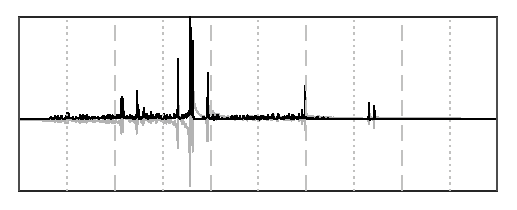
\includegraphics[width=0.95\textwidth,keepaspectratio]{images/PM_stages/pm_stages_1.eps}
    %     \caption{Original basis functions}
    %     \label{fig:PM_stages:basis functions}\vspace{0.2\baselineskip}
    % \end{subfigure}&
    % \begin{subfigure}[c]{0.315\textwidth}
    %     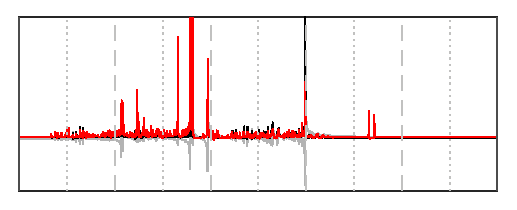
\includegraphics[width=0.95\textwidth,keepaspectratio]{images/PM_stages/pm_stages_2.eps}
    %     \caption{Modulated basis functions}
    %     \label{fig:PM_stages:modulated}\vspace{0.2\baselineskip}
    % \end{subfigure}&
    % \begin{subfigure}[c]{0.315\textwidth}
    %     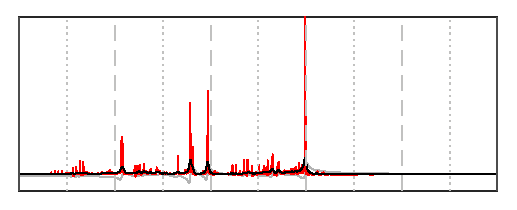
\includegraphics[width=0.95\textwidth,keepaspectratio]{images/PM_stages/pm_stages_3.eps}
    %     \caption{Voigt lineshape}
    %     \label{fig:PM_stages:B0 inhomogeneities}\vspace{0.2\baselineskip}
    % \end{subfigure}\\[25pt]
    % \begin{subfigure}[c]{0.315\textwidth}
    %     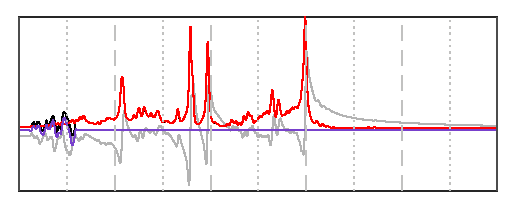
\includegraphics[width=0.95\textwidth,keepaspectratio]{images/PM_stages/pm_stages_4.eps}
    %     \caption{Residual Water}
    %     \label{fig:PM_stages:lineshape}\vspace{0.2\baselineskip}
    % \end{subfigure}&
    % \begin{subfigure}[c]{0.315\textwidth}
    %     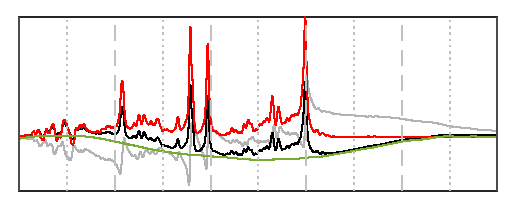
\includegraphics[width=0.95\textwidth,keepaspectratio]{images/PM_stages/pm_stages_5.eps}
    %     \caption{Baseline}
    %     \label{fig:PM_stages:phi1}\vspace{0.2\baselineskip}
    % \end{subfigure}&
    % \begin{subfigure}[c]{0.315\textwidth}
    %     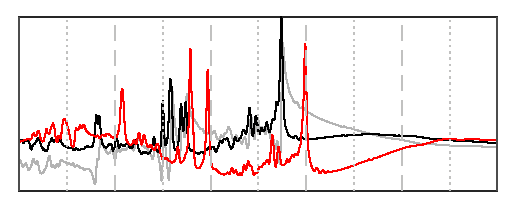
\includegraphics[width=0.95\textwidth,keepaspectratio]{images/PM_stages/pm_stages_6.eps}
    %     \caption{Frequency Shift}
    %     \label{fig:PM_stages:phi0}\vspace{0.2\baselineskip}\vspace{0.2\baselineskip}
    % \end{subfigure}\\[25pt]
    % \begin{subfigure}[c]{0.315\textwidth}
    %     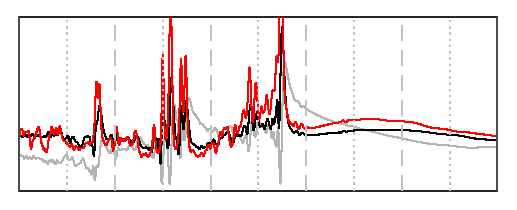
\includegraphics[width=0.95\textwidth,keepaspectratio]{images/PM_stages/pm_stages_7.eps}
    %     \caption{Eddy currents}
    %     \label{fig:PM_stages:fshift}\vspace{0.2\baselineskip}
    % \end{subfigure}&
    % \begin{subfigure}[c]{0.315\textwidth}
    %     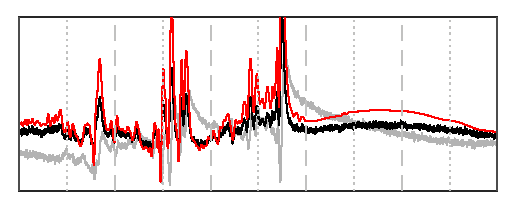
\includegraphics[width=0.95\textwidth,keepaspectratio]{images/PM_stages/pm_stages_8.eps}
    %     \caption{Noise}
    %     \label{fig:PM_stages:SNR}\vspace{0.2\baselineskip}
    % \end{subfigure}&
    % \begin{subfigure}[c]{0.315\textwidth}
    %     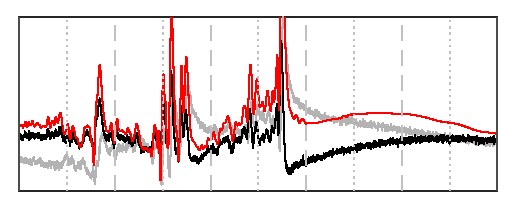
\includegraphics[width=0.95\textwidth,keepaspectratio]{images/PM_stages/pm_stages_9.eps}
    %     \caption{First-order phase}
    %     \label{fig:PM_stages:residual water}\vspace{0.2\baselineskip}
    % \end{subfigure}\\[25pt]
    % \begin{subfigure}[c]{0.315\textwidth}
    %     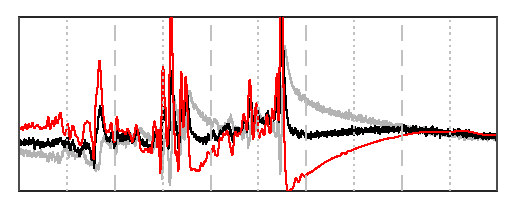
\includegraphics[width=0.95\textwidth,keepaspectratio]{images/PM_stages/pm_stages_10.eps}
    %     \vspace{0.5pt}
    %     \caption{Zero-order phase}
    %     \label{fig:PM_stages:baseline}
    % \end{subfigure}&
    % \begin{subfigure}[c]{0.315\textwidth}
    %     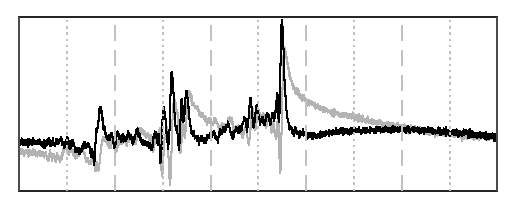
\includegraphics[width=0.95\textwidth,keepaspectratio]{images/PM_stages/pm_stages_11.eps}
    %     \vspace{0.5mm}
    %     \caption{Generated spectrum}
    %     \label{fig:PM_stages:generated spectrum}
    % \end{subfigure}&
    % \begin{subfigure}[c]{0.315\textwidth}
    %     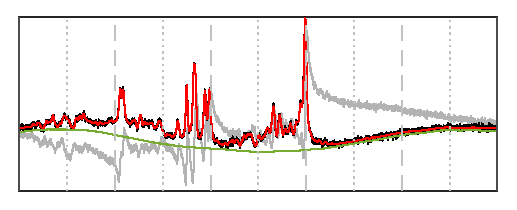
\includegraphics[width=0.95\textwidth,keepaspectratio]{images/PM_stages/pm_stages_12.eps} \smallskip
    %     \caption{Pre-processed spectrum}
    %     \label{fig:PM_stages:corrected}
    % \end{subfigure}
    % \end{tabular}
    \includegraphics[width=\textwidth,keepaspectratio]{images/compiled_figures/MRS_Sim_Figure_1_PM_stages_1.png}
    \caption{This is a step-by-step progression through the physics model. The real and imaginary components are depicted in black and gray, respectively. The red line includes only the metabolites and the offsets from the preceding steps. \ref{fig:PM_stages:generated spectrum} shows the final spectrum with all artifacts applied. \ref{fig:PM_stages:corrected} is the pre-processed spectrum with the phase and frequency shifts removed.}
    \label{fig:PM compilation}
\end{figure}


\subsubsection{Basis Functions}
MRI, and its derivatives, are spatially resolved imaging modalities. MR pixels and voxels represent 3D volumes with a spatial distribution, as shown in Fig. \ref{fig:spatial voxel}, and needs to be accounted for in simulations. The importance of spatial localization led to selecting Landheer \etal's Magnetic Resonance Spectrum Simulator (MARSS)\cite{Landheer2021} software package for simulating the default basis functions provided with this simulator. MARSS produces high-fidelity outputs by simulating 128 points in each direction, accurately capturing the spatial nature the RF pulses and slice-selective gradients. Using vendor-specific pulse sequences, MARSS can simulate individual or summed spins for a large number of common brain metabolites including macromolecules and lipids.% vendor-specific basis functions making it easy to use for new simulations. 
% The default basis functions are stored as individual spins for each metabolite allowing fine-detailed artifacts to be included. %for these metabolites can be simulated with PRESS and STEAM sequences. Custom basis functions can also be simulated with various metabolites, T1 and T2 relaxations, and specialized pulse sequences, e.g. editing sequences, (semi-)LASER, etc.
 
\begin{figure}[b]
    \centering
    % \begin{tabular}[b]{>{\centering}b{0.315\textwidth}>{\centering}b{0.315\textwidth}>{\centering}b{0.315\textwidth}}
    %     \centering
    %     \begin{subfigure}[c]{0.315\textwidth}
    %         \centering
    %         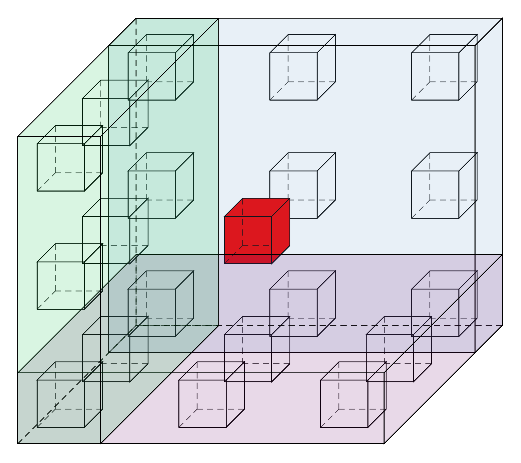
\includegraphics[width=5cm,keepaspectratio]{images/spatial_localization.eps}
    %         \caption{Intravoxel localization}
    %         \label{fig:spatial voxel}
    %     \end{subfigure} & 
    %     \begin{subfigure}[c]{0.315\textwidth}
    %         \centering
    %         \def\svgwidth{5cm}
    %         \input{images/B0_inhomogeneity_cube.eps_tex}
    %         \caption{Intravoxel spatial distribution of $B_0$ with minor distortions}
    %         \label{fig:spatial B0}
    %     \end{subfigure} &
    %     \begin{subfigure}[c]{0.315\textwidth}
    %         \centering
    %         \def\svgwidth{5cm}
    %         \input{images/B0_inhomogeneity_cube_severe_distortion.eps_tex}
    %         \caption{Spatial distribution of $B_0$ with major distortions}
    %         \label{fig:spatial B0 severe}
    %     \end{subfigure}
    % \end{tabular}
    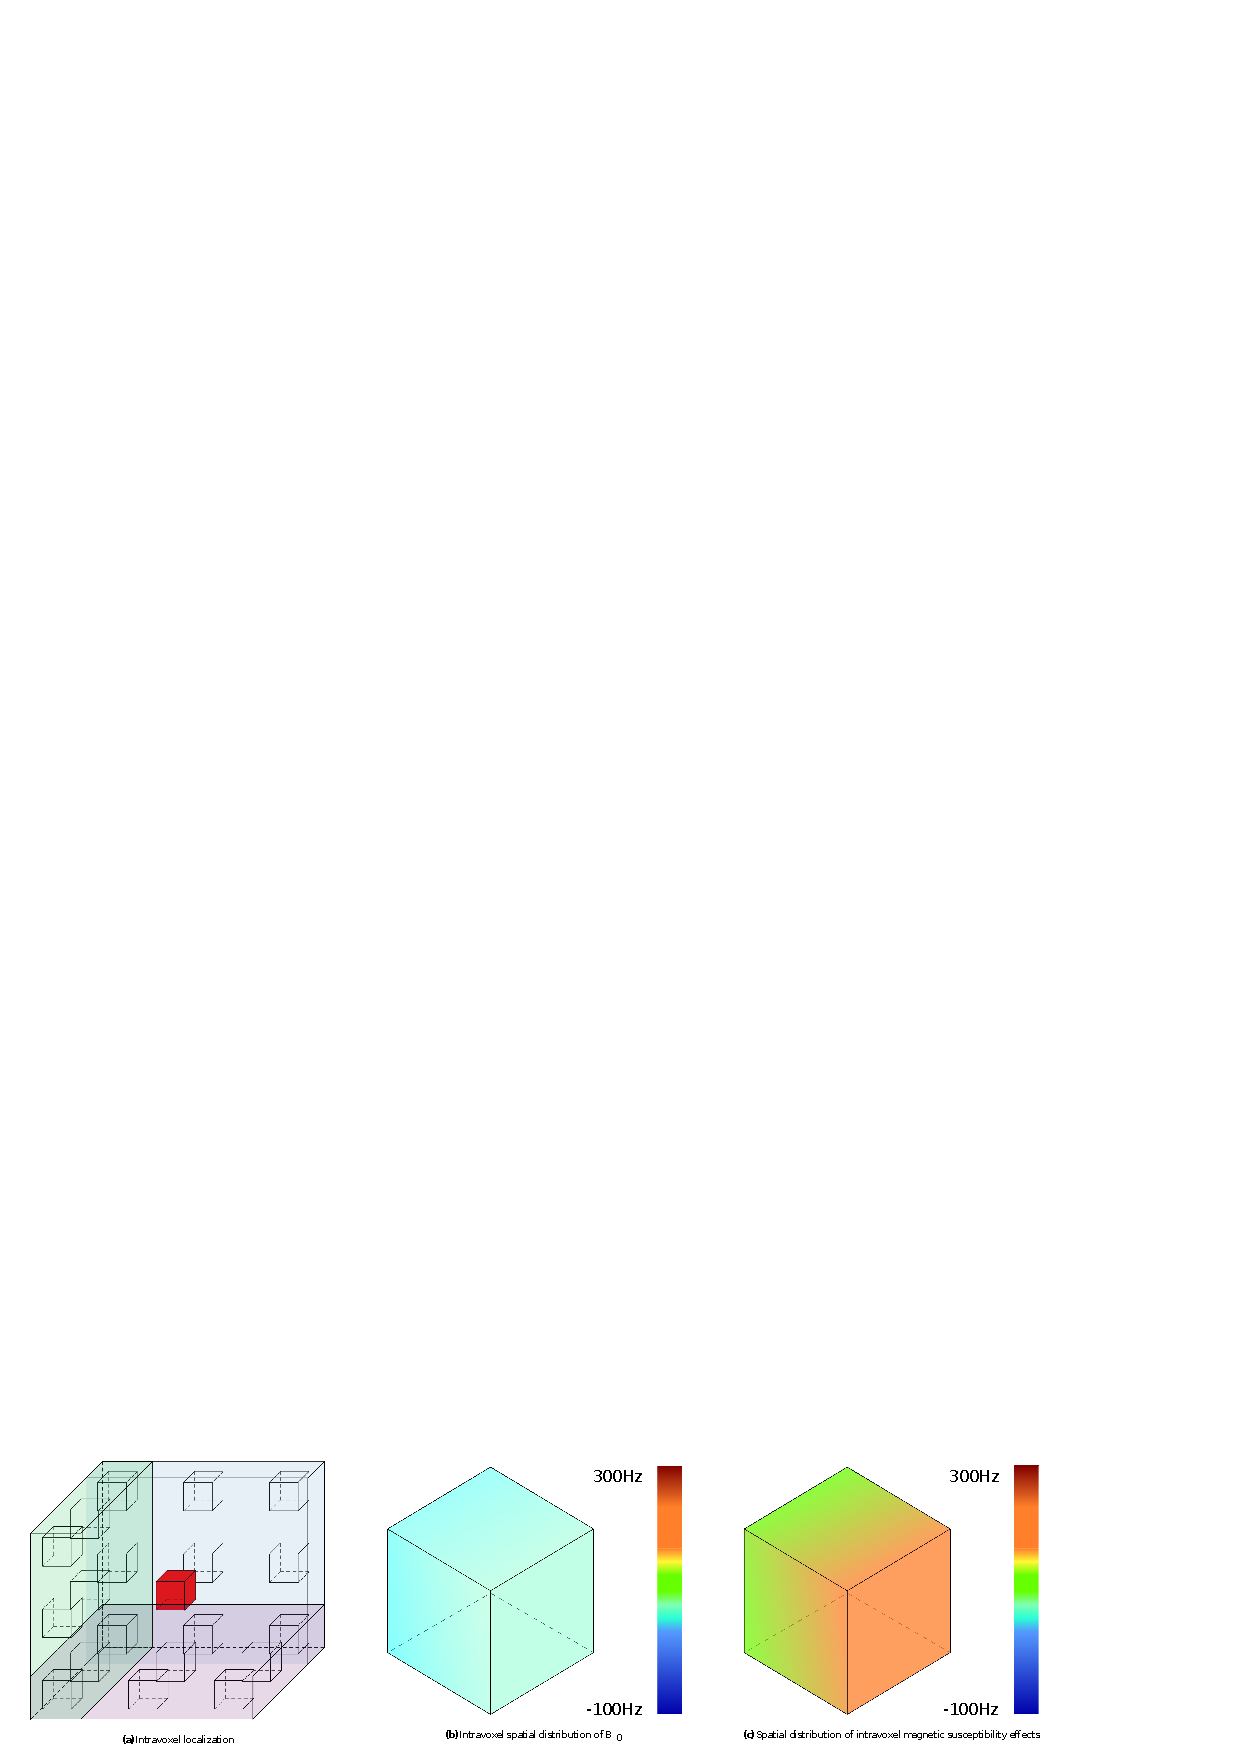
\includegraphics[width=\textwidth, keepaspectratio]{images/compiled_figures/MRS-Sim_Figure2_Spatial_localization.png}
    \caption{Voxels are often treated as singularities, meaning the entire volume is considered to be a single point like the red box in the center. Accounting for these intravoxel distributions leads to more accurate and more realistic simulations. \ref{fig:spatial voxel} highlights the spatial nature of voxels while \ref{fig:spatial B0} and \ref{fig:spatial B0 severe} show different levels of intravoxel $B_0$ inhomogeneity.}
    \label{fig:intravoxel localization}
\end{figure}

 
% \paragraph{Macromolecules and Lipids}
% Current spectral fitting methods for modeling MM and lipid signals are based on creating a group of curves that resemble clinical data but are not informed by any underlying physical phenomenon. Each fitting package contains their own set of basis functions for modeling these regions. Until this knowledge gap is filled and better simulation methods are developed, this work will use pre-generated basis functions from Osprey\cite{Oeltzschner2020}.% that were resampled to match the simulated basis functions from MARSS.
 
\subsubsection{Amplitude Modulation}
For this framework, comprehensive ranges including physiological and pathological values were adapted from the meta-analysis by Gudmundson \etal\cite{Gudmundson2023}. Near\cite{Near2021} and Larsen\cite{Larsen2021} discuss how non-trivial the choice of reference metabolite is with respect to quantification and interpretability. Therefore, the default ranges are in units of milimolar (mM) which allows any reference to be used. More specific information can be found in the MARSS user manual.
% Metabolite quantities produced during spectral fitting are of an arbitrary scale. Comparing these quantities with a standard reference puts them into context. In vivo proton scans generally use an internal reference metabolite for relative quantification. Creatine is the default metabolite because its concentration is relatively stable. As a result, concentrations maps are generally reported as ratios with respect to creatine and all amplitude values in this model are defined \textit{wrt} creatine as the default. For this framework, comprehensive ranges including physiological and pathological values were adapted from the meta-analysis by Gudmundson \etal\cite{Gudmundson2023}. 
%These ranges were then expanded to include values observed in in vivo scans from a private glioma dataset. In keeping in line with the LCModel, the expected concentrations ranges represent the scaling factors needed for spectral fitting instead of the ratios of peak integrals or peak heights.
 
\subsubsection{Lineshape Profiles}\label{subsubsec:lineshapes}
The Voigt lineshape profile is the most commonly used in spectral fitting as it most closely matches in vivo data.
% In spectral fitting, the Voigt lineshape profile is the most commonly used as it most closely matches clinical data. 
It is a combination of a Lorentzian and a Gaussian and is used in various fitting packages, such as LCModel\cite{Provencher2001}, TARQUIN\cite{Wilson2011}, jMRUI\cite{Stefan2009}, and Osprey\cite{Oeltzschner2020}. For completeness, it is also possible to specify either a purely Lorentzian or a purely Gaussian lineshape. 
Individual Lorentzian and Gaussian values can be assigned to each moiety or metabolite separately, depending on the desired level of granularity. At the most basic level, each metabolite is assigned a Lorentzian value while a single Gaussian value is applied to the set of metabolites and a second value can be applied to the macromolecules and lipids. Standard practice from the aforementioned software packages assigns a single Lorentzian value to each metabolite, instead of each moiety. However, experimental results from Wyss \etal\cite{Wyss2018} can be used, which characterized moiety-level T2 relaxation values for metabolites in three brain regions at 3T. Information for some metabolites can be supplemented by the meta-analysis from Gudmundson \etal\cite{Gudmundson2023}. As more metabolites are characterized, new information can be added to the model. A detailed table will be provided in the appendix with the current information, however a digital version that can be updated will also be maintained in the repository.
 
\subsubsection{$B_0$ Inhomogeneities}
% Lower and higher order shimming procedures homogenize the magnetic field in the target volume to different degrees. However, certain regions of the brain, such as the prefrontal cortex or deep brain structures like the thalamus or basal ganglia, are more difficult to shim and therefore suffer from large magnetic susceptibility effects, resulting in significant lineshape distortions. Fig. \ref{fig:spatial B0} shows the normal, subtle $B_0$ changes across the volume of a spectroscopy voxel while Fig. \ref{fig:spatial B0 severe} illustrates these high susceptibility effects. In such cases, spectra from these regions exhibit significant lineshape distortions which cannot be adequately characterized using idealized lineshape profiles. Fig. \ref{fig:B0 effects} shows the result of high susceptibility effects on lineshapes.

% \begin{figure}
    \centering
    \begin{subfigure}{0.32\textwidth}
        \centering
        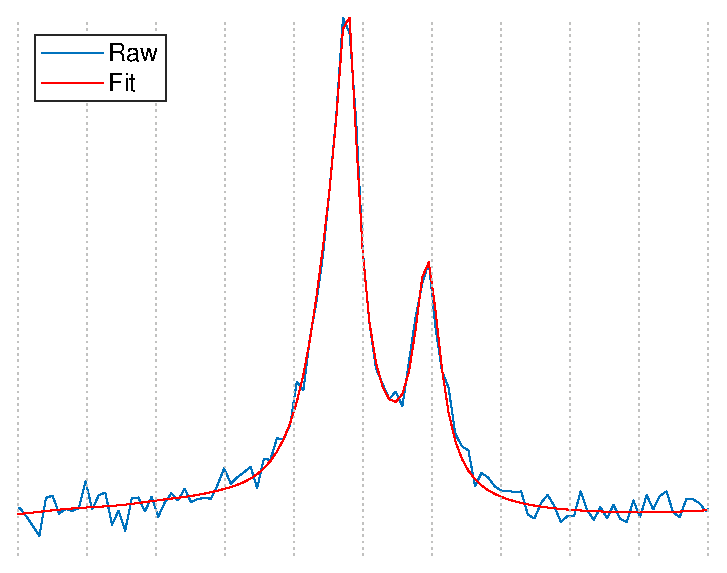
\includegraphics[width=0.95\textwidth,keepaspectratio]{images/b0_peaks/no_B0.eps}
        \caption{Spectral peaks without $B_0$ inhomogeneities ($\mu = 0$Hz)}
        \label{subfig:without B0}        
    \end{subfigure}
    \begin{subfigure}{0.32\textwidth}
        \centering
        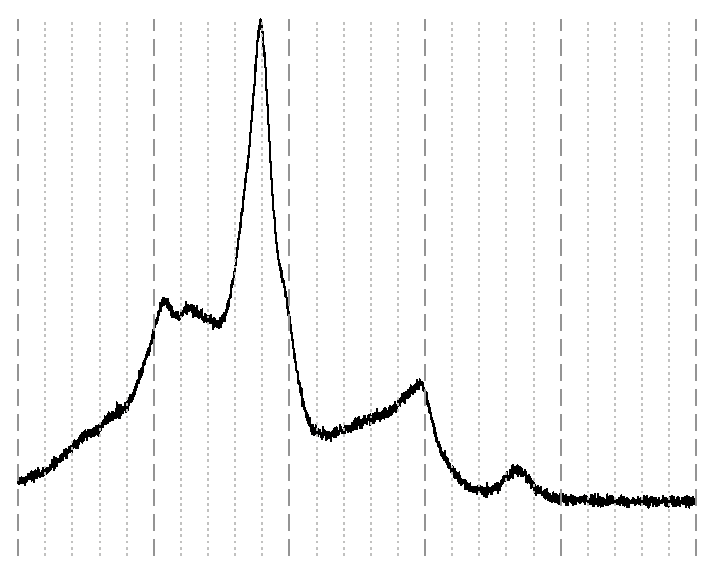
\includegraphics[width=0.95\textwidth,keepaspectratio]{images/b0_peaks/some_B0.eps}
        \caption{Spectral peaks with moderate $B_0$ inhomogeneities ($\mu = 75$Hz)}
        \label{subfig:some B0}        
    \end{subfigure}
    \begin{subfigure}{0.32\textwidth}
        \centering
        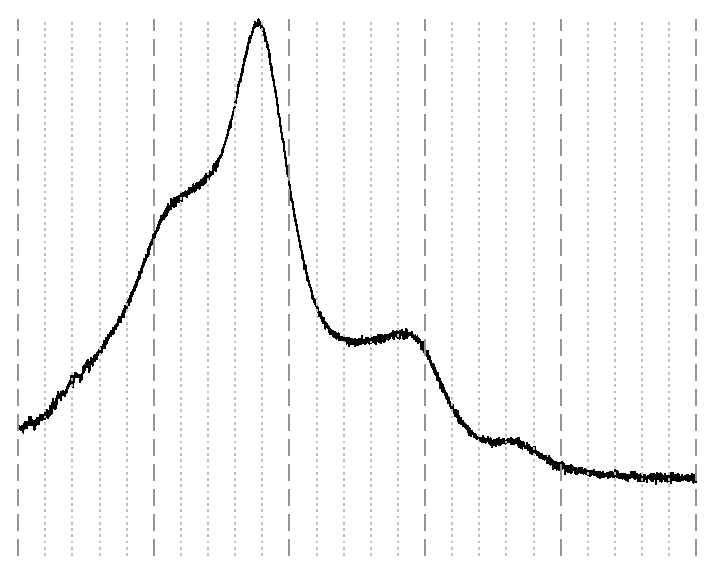
\includegraphics[width=0.95\textwidth,keepaspectratio]{images/b0_peaks/with_B0.eps}
        \caption{Spectral peaks with severe $B_0$ inhomogeneities ($\mu = 175$Hz)}
        \label{subfig:with B0}        
    \end{subfigure}
    \caption{These samples show the effects that can be modeled using the 3D $B_0$ field simulator. In \ref{subfig:without B0}, the spectral peaks have a purely Lorentzian lineshape. In \ref{subfig:some B0}, the lineshape is now Voigtian because the Gaussian term has been added back by the 3D $B_0$ field simulator. In \ref{subfig:with B0}, severe heterogeneities are modeled which produce extremely broad line widths. All three plots use the same x- and y-axes. The observed offsets are caused by the line broadening.}
    \label{fig:B0 effects}
\end{figure}


Small $B_0$ inhomoegeneities are, in general, sufficiently modeled by the Gaussian term of the Voigt lineshape. However, to simulate more severe distortions from large inhomogeneities, a $B_0$ field volume needs to be modeled and applied to the basis functions. Fig. \ref{fig:intravoxel localization} illustrates the difference between small and severe $B_0$ inhomogeneities. Fig. \ref{fig:spatial B0} shows the normal, subtle $B_0$ changes across the volume of a spectroscopy voxel while Fig. \ref{fig:spatial B0 severe} illustrates these high susceptibility effects. In such cases, spectra from these regions exhibit significant lineshape distortions which cannot be adequately characterized using idealized lineshape profiles. Fig. \ref{fig:B0 effects} shows the result of high susceptibility effects on lineshapes.

\begin{figure}
    \centering
    \begin{subfigure}{0.32\textwidth}
        \centering
        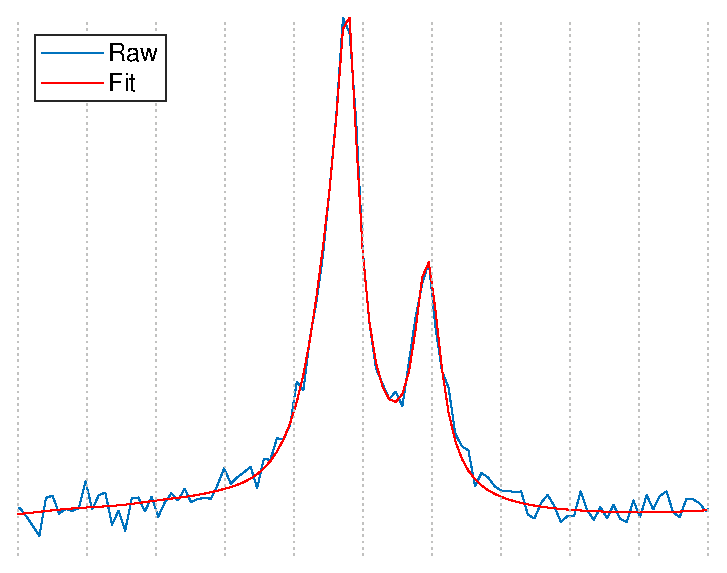
\includegraphics[width=0.95\textwidth,keepaspectratio]{images/b0_peaks/no_B0.eps}
        \caption{Spectral peaks without $B_0$ inhomogeneities ($\mu = 0$Hz)}
        \label{subfig:without B0}        
    \end{subfigure}
    \begin{subfigure}{0.32\textwidth}
        \centering
        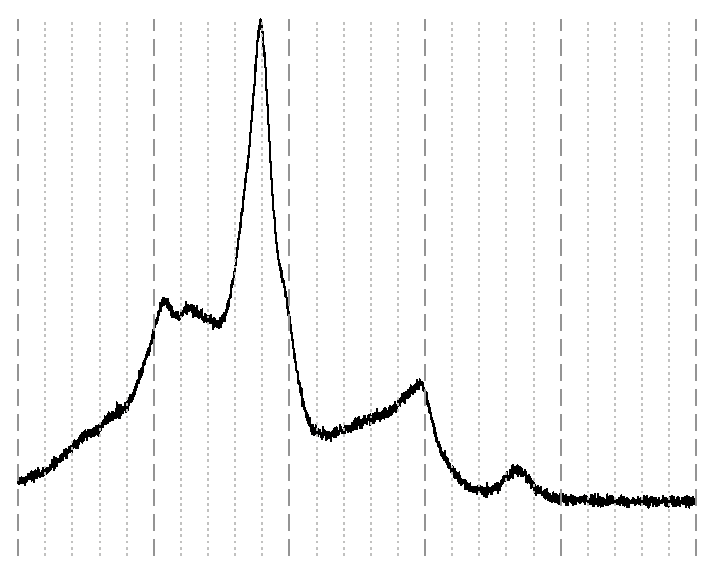
\includegraphics[width=0.95\textwidth,keepaspectratio]{images/b0_peaks/some_B0.eps}
        \caption{Spectral peaks with moderate $B_0$ inhomogeneities ($\mu = 75$Hz)}
        \label{subfig:some B0}        
    \end{subfigure}
    \begin{subfigure}{0.32\textwidth}
        \centering
        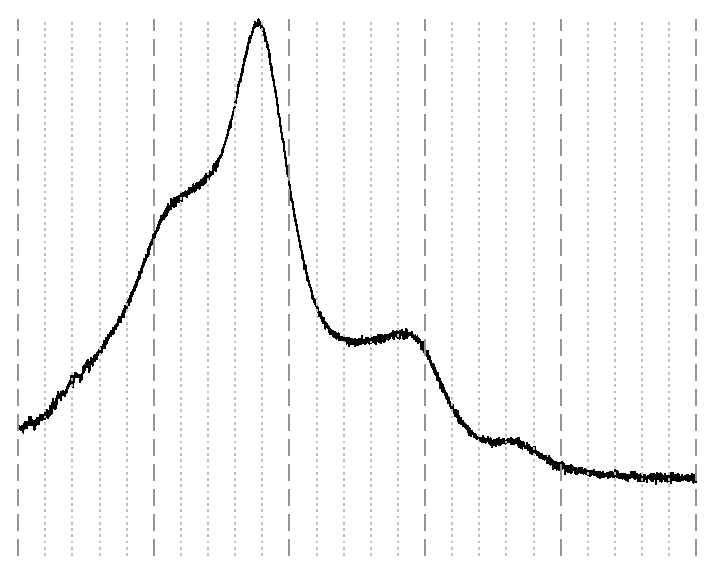
\includegraphics[width=0.95\textwidth,keepaspectratio]{images/b0_peaks/with_B0.eps}
        \caption{Spectral peaks with severe $B_0$ inhomogeneities ($\mu = 175$Hz)}
        \label{subfig:with B0}        
    \end{subfigure}
    \caption{These samples show the effects that can be modeled using the 3D $B_0$ field simulator. In \ref{subfig:without B0}, the spectral peaks have a purely Lorentzian lineshape. In \ref{subfig:some B0}, the lineshape is now Voigtian because the Gaussian term has been added back by the 3D $B_0$ field simulator. In \ref{subfig:with B0}, severe heterogeneities are modeled which produce extremely broad line widths. All three plots use the same x- and y-axes. The observed offsets are caused by the line broadening.}
    \label{fig:B0 effects}
\end{figure}


In general, this approach mirrors Li \etal\cite{Li2015} in which the basis functions are modulated by the $B_0$ field map, but in the implmenetation the $B_0$ field map is simulated rather than acquired. As with MARSS, Li \etal\ suggests using multiple points in each direction instead of a single value per voxel. The exact number of points used in each direction is described by the size of the spectroscopy voxel divided by the size of an anatomical imaging voxel. %The default values assume sizes of 10cm$^3$ and 0.5cm$^3$ respectively, which results in $20^3$ simulation points. 
% However, a
Any cuboidal shape, rectangular or otherwise, can be modeled. The $B_0$ field is defined by four variables: $\pm dx$, $\pm dy$, $\pm dz$, and $\mu$. $dx, dy,$ and $dz$ describe half of the change in $B_0$ in their respective axis from the voxel's center and $\mu$ is the mean of the entire voxel. A linear $B_0$ gradient is assumed, but other shapes can be implemented. The first section in the supplement provides a more detailed explanation for how the $B_0$ is simulated.

% Lower and higher order shimming procedures homogenize the magnetic field in the target volume to different degrees. However, certain regions of the brain, such as the prefrontal cortex or deep brain structures like the thalamus or basal ganglia, are more difficult to shim and therefore suffer from large magnetic susceptibility effects, resulting in significant lineshape distortions. Fig. \ref{fig:spatial B0} shows the normal, subtle $B_0$ changes across the volume of a spectroscopy voxel while Fig. \ref{fig:spatial B0 severe} illustrates these high susceptibility effects. In such cases, spectra from these regions exhibit significant lineshape distortions which cannot be adequately characterized using idealized lineshape profiles. Fig. \ref{fig:B0 effects} shows the result of high susceptibility effects on lineshapes.

% \begin{figure}
    \centering
    \begin{subfigure}{0.32\textwidth}
        \centering
        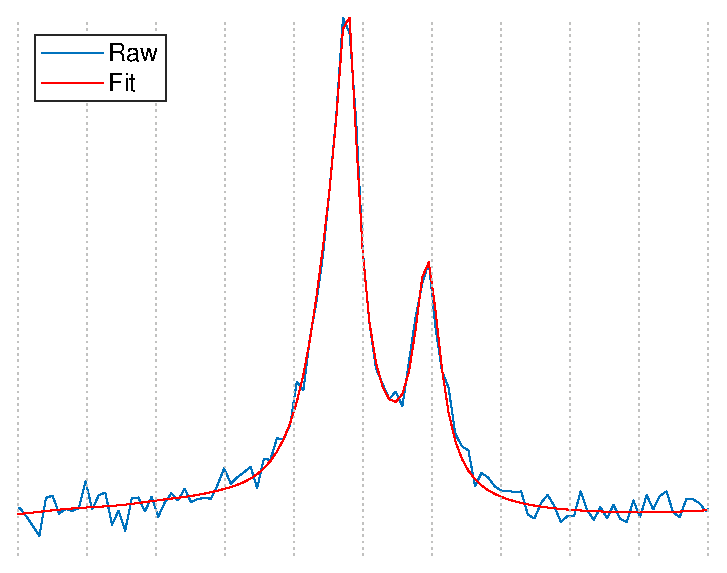
\includegraphics[width=0.95\textwidth,keepaspectratio]{images/b0_peaks/no_B0.eps}
        \caption{Spectral peaks without $B_0$ inhomogeneities ($\mu = 0$Hz)}
        \label{subfig:without B0}        
    \end{subfigure}
    \begin{subfigure}{0.32\textwidth}
        \centering
        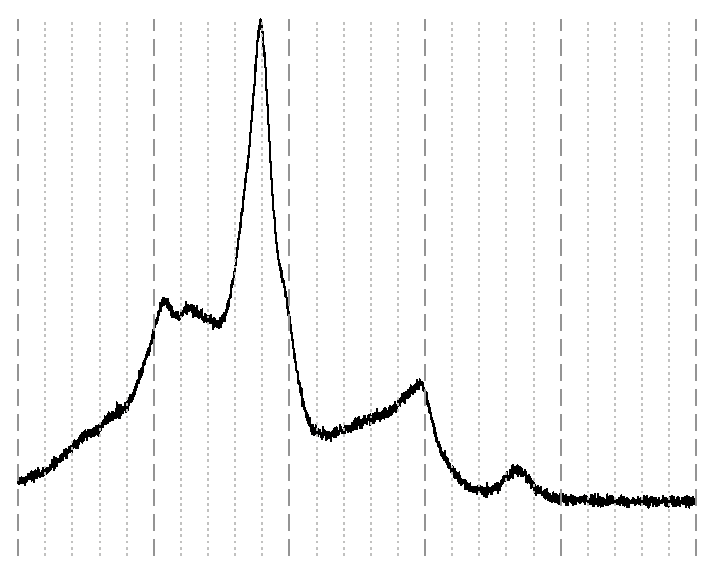
\includegraphics[width=0.95\textwidth,keepaspectratio]{images/b0_peaks/some_B0.eps}
        \caption{Spectral peaks with moderate $B_0$ inhomogeneities ($\mu = 75$Hz)}
        \label{subfig:some B0}        
    \end{subfigure}
    \begin{subfigure}{0.32\textwidth}
        \centering
        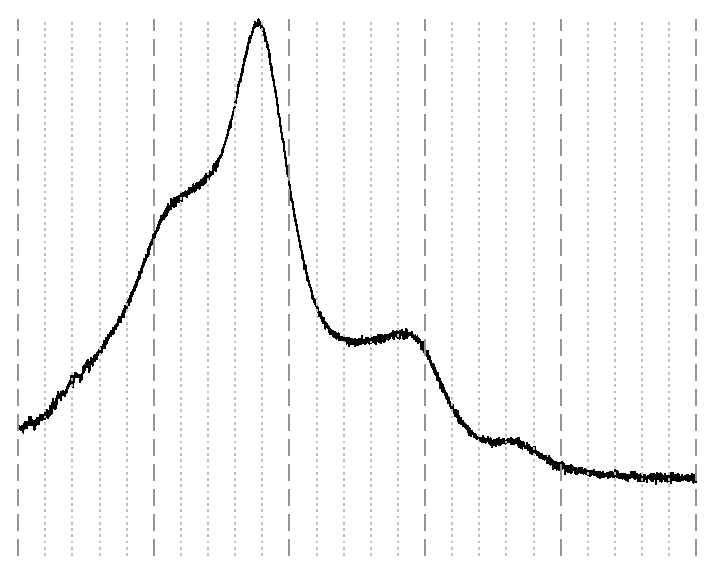
\includegraphics[width=0.95\textwidth,keepaspectratio]{images/b0_peaks/with_B0.eps}
        \caption{Spectral peaks with severe $B_0$ inhomogeneities ($\mu = 175$Hz)}
        \label{subfig:with B0}        
    \end{subfigure}
    \caption{These samples show the effects that can be modeled using the 3D $B_0$ field simulator. In \ref{subfig:without B0}, the spectral peaks have a purely Lorentzian lineshape. In \ref{subfig:some B0}, the lineshape is now Voigtian because the Gaussian term has been added back by the 3D $B_0$ field simulator. In \ref{subfig:with B0}, severe heterogeneities are modeled which produce extremely broad line widths. All three plots use the same x- and y-axes. The observed offsets are caused by the line broadening.}
    \label{fig:B0 effects}
\end{figure}


% Small $B_0$ inhomoegeneities are, in general, sufficiently modeled by the Gaussian term of the Voigt lineshape. However, to simulate more severe distortions, a $B_0$ field volume needs to be modeled and applied to the basis functions. In general, this approach mirrors Li \etal\cite{Li2015}, but the $B_0$ field map is simulated rather than acquired. As with MARSS, Li \etal\ suggests using multiple points in each direction instead of a single value per voxel. The exact number of points used in each direction is described by the size of the spectroscopy voxel divided by the size of an anatomical imaging voxel. The default values assume sizes of 10cm$^3$ and 0.5cm$^3$ respectively, which results in $20^3$ simulation points. However, any cuboidal shape, rectangular or otherwise, can be modeled. The $B_0$ field is defined by four variables, all of which are mean offsets: $\pm dx$, $\pm dy$, $\pm dz$, and $\mu$. $dx, dy,$ and $dz$ describe half of the change in $B_0$ in their respective direction from the voxel's center and $\mu$ is the mean of the entire voxel. 

\begin{figure}[b!]
    \centering
    \begin{tabular}[l]{cc}
    \begin{subfigure}{0.49\textwidth}
        \centering
        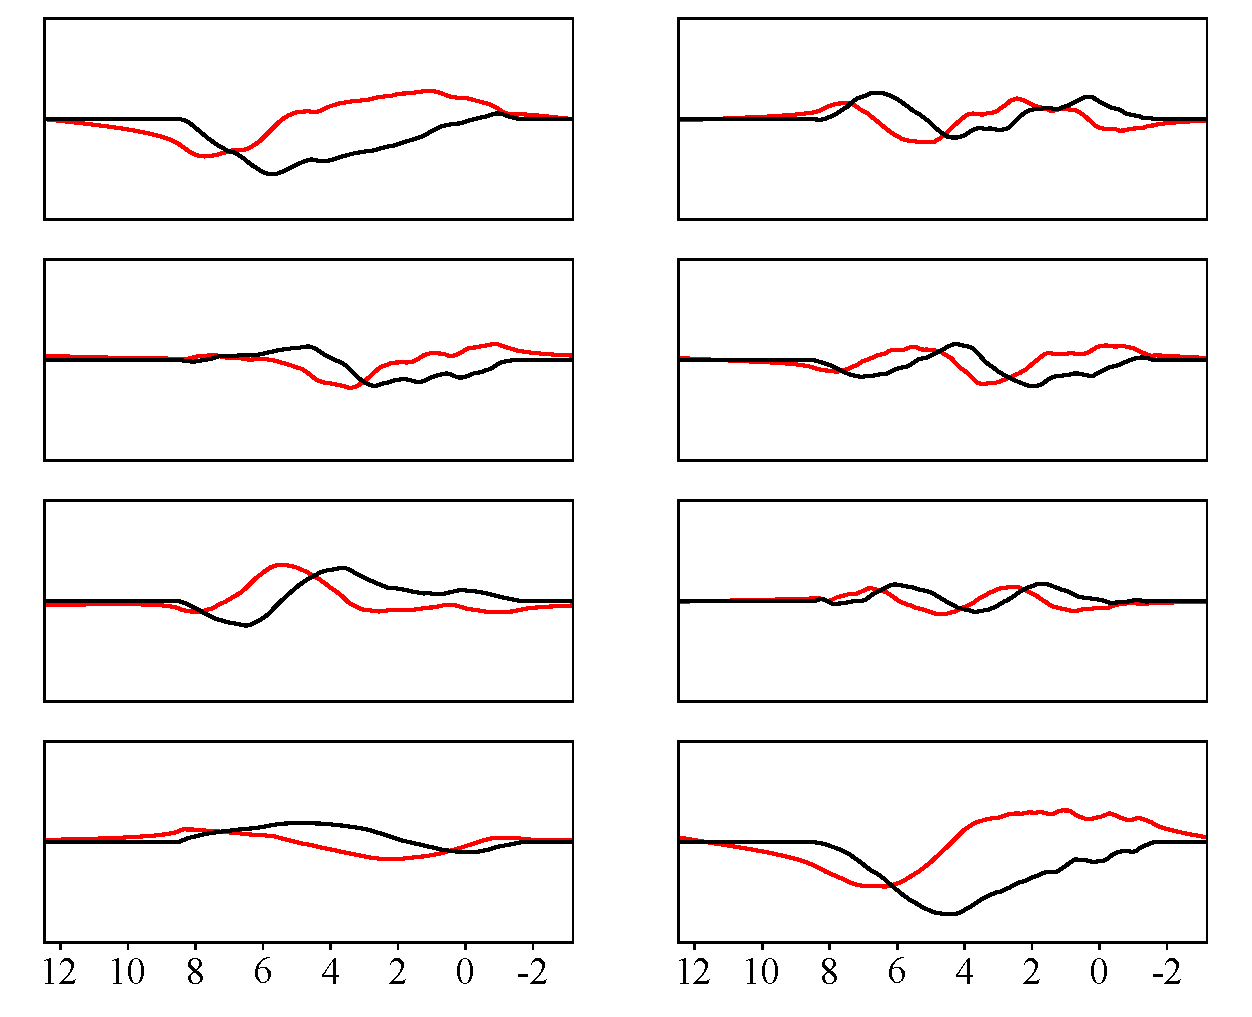
\includegraphics[width=0.95\textwidth,keepaspectratio]{images/random_walks/baseline_walks_edited.eps}
        \caption{Simulated baselines}
        \label{fig:baseline_region}
    \end{subfigure} &
    
    \begin{subfigure}{0.49\textwidth}
        \centering
        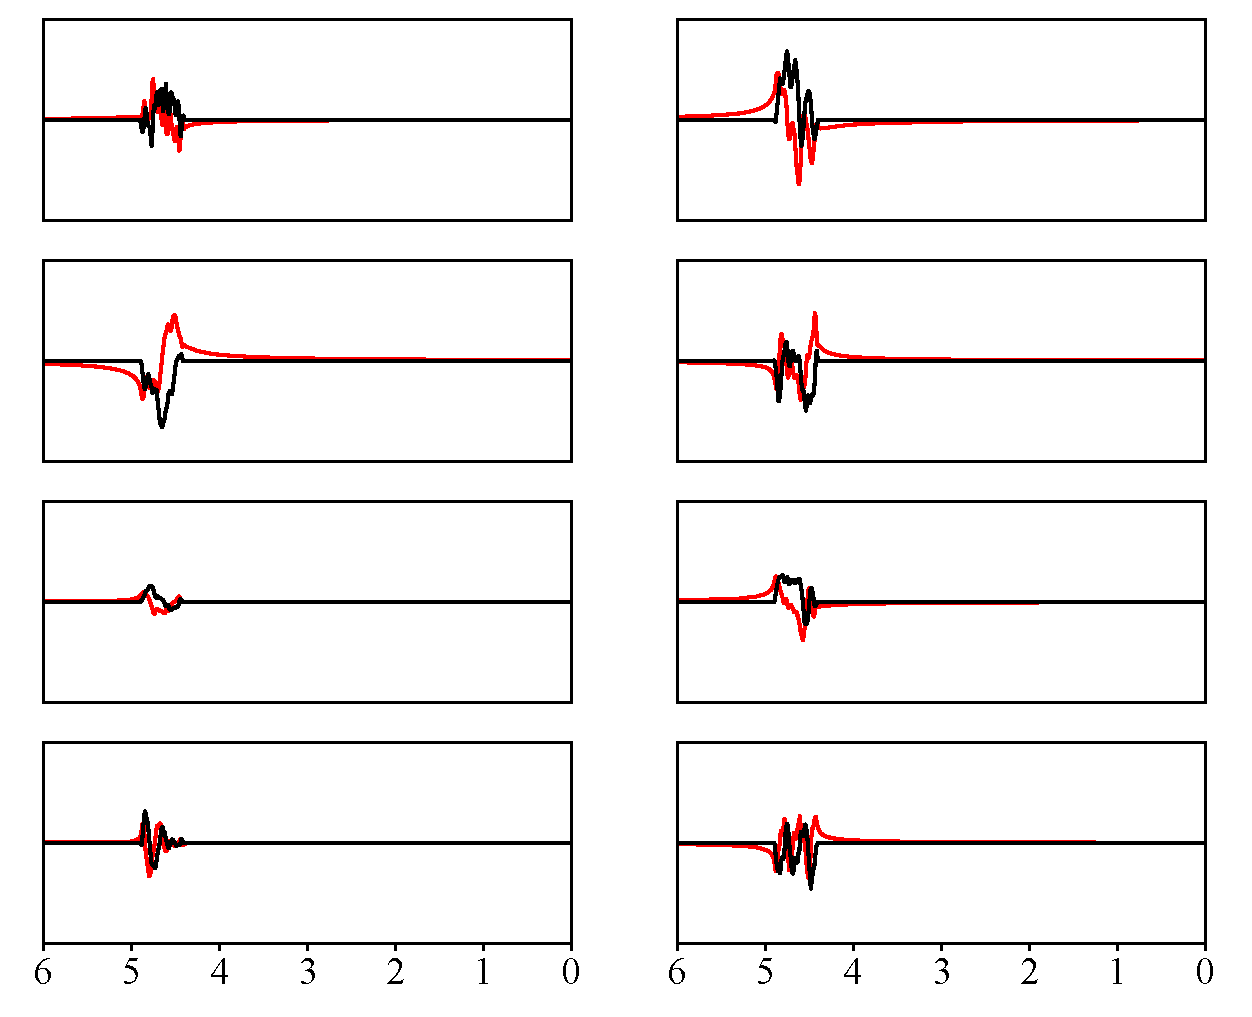
\includegraphics[width=0.95\textwidth,keepaspectratio]{images/random_walks/reswater_walks_edited.eps}
        \caption{Simulated residual water}
        \label{fig:reswater_region}
    \end{subfigure}
    \end{tabular}
    \caption{Simulated  samples of spectral baselines and residual water regions using the pseudo-random bounded walk generator. The blue lines are the raw simulations. The red lines are the smoothed versions that are then returned and applied to the simulated spectra.}
    \label{fig:random walk generator}
\end{figure}

\begin{algorithm}[t!]
\caption{Smoothed Bounded Pseudo-Random Walk} \label{alg:smoothed bounded pseudo-random walk}
\begin{algorithmic}[1]
\Require $start$: ppm start value, $end$: ppm end value, $std$: standard deviation of the random noise, $lower\_bound$: lower bound of the walk, $upper\_bound$: upper bound of the walk, $length$: length of the walk
% \Ensure $rand\_walk$: bounded pseudo-random walk
\end{algorithmic}

\textbf{Function} SmoothedBoundedPseudoRandomWalk($start, end, std, lower\_bound, upper\_bound, length, window\_size$)
% \Function{BoundedPseudoRandomWalk}{$start, end, std, lower\_bound, upper\_bound, length$}
\begin{algorithmic}[1]
\State $bounds = upper\_bound - lower\_bound$
\Statex Generate raw random walk
\State $rand = \text{generate\_random\_array}(size=length, std=std)$
\State $rand = \text{cumsum}(rand, dim=-1)$

\Statex Calculate the trend line
\State $rand\_trend\_lines = \text{generate\_trend\_array}(start, end, length)$

\Statex Calculate the difference between the random steps and the trend line
\State $rand\_deltas = rand - rand\_trend\_lines$
\Statex Normalize the delta array
\State $delta\_range = bounds \div (rand\_deltas.max() - rand\_deltas.min())$
\State $rand\_deltas = rand\_deltas * delta\_range$

\Statex Adjust delta array if it exceeds \textit{bounds}
\State $rand\_deltas = conditional\_adjustment(rand\_deltas)$
\Statex Calculate the final random walk
\State $random\_walk = trend\_lines + rand\_deltas$

\Statex Smooth using a uniform smoothing kernel
% \State $kernel\_size $
\State $random\_walk = \text{average\_smoothing}(random\_walk, kernel\_size=window\_size * length)$

\Statex \Return $random\_walk$ %trend\_lines + rand_deltas$
% \EndFunction
\end{algorithmic}
\end{algorithm}

 
\subsubsection{Baseline and Residual Water}


Currently, the underlying physical phenomena that induce spectral baseline offsets are poorly understood. In fact, there is no physics-based model for simulating these offsets. Similarly, the residual water region is also poorly characterized. Therefore, a naive random model can be used in conjunction with observed constraints to approximate what is expected in vivo. This work proposes a smoothed, pseudo-random, bounded walk generator for both the broad spectral baseline and the more irregular residual water region. The approach is elaborated on in Algorithm \ref{alg:smoothed bounded pseudo-random walk}. Customizable profiles were developed for each artifact to more closely approximate what is expected in vivo. Immense variety of outputs can be achieved by randomly sampling the parameters from distributions instead of using fixed values. Once simulated, they are resampled to match the ppm range of acquired data and the order of magnitude is matched to the spectra. The Hilbert transform is then used to generate the corresponding complex component before being added to the FID. As shown in Fig. \ref{fig:random walk generator}, this generator produces very different outputs depending on the specified configurations. Fig. \ref{fig:baseline_region} shows very broad, smooth lines while Fig. \ref{fig:reswater_region} shows highly irregular lines that closely resemble residual water regions. All outputs are then scaled to modulate the impact on the final spectra. A more detailed exploration of this algorithm and the effects of each parameter are presented in the supplement for baseline and residual water simulations.

% \begin{algorithm}[t!]
\caption{Smoothed Bounded Pseudo-Random Walk} \label{alg:smoothed bounded pseudo-random walk}
\begin{algorithmic}[1]
\Require $start$: ppm start value, $end$: ppm end value, $std$: standard deviation of the random noise, $lower\_bound$: lower bound of the walk, $upper\_bound$: upper bound of the walk, $length$: length of the walk
% \Ensure $rand\_walk$: bounded pseudo-random walk
\end{algorithmic}

\textbf{Function} SmoothedBoundedPseudoRandomWalk($start, end, std, lower\_bound, upper\_bound, length, window\_size$)
% \Function{BoundedPseudoRandomWalk}{$start, end, std, lower\_bound, upper\_bound, length$}
\begin{algorithmic}[1]
\State $bounds = upper\_bound - lower\_bound$
\Statex Generate raw random walk
\State $rand = \text{generate\_random\_array}(size=length, std=std)$
\State $rand = \text{cumsum}(rand, dim=-1)$

\Statex Calculate the trend line
\State $rand\_trend\_lines = \text{generate\_trend\_array}(start, end, length)$

\Statex Calculate the difference between the random steps and the trend line
\State $rand\_deltas = rand - rand\_trend\_lines$
\Statex Normalize the delta array
\State $delta\_range = bounds \div (rand\_deltas.max() - rand\_deltas.min())$
\State $rand\_deltas = rand\_deltas * delta\_range$

\Statex Adjust delta array if it exceeds \textit{bounds}
\State $rand\_deltas = conditional\_adjustment(rand\_deltas)$
\Statex Calculate the final random walk
\State $random\_walk = trend\_lines + rand\_deltas$

\Statex Smooth using a uniform smoothing kernel
% \State $kernel\_size $
\State $random\_walk = \text{average\_smoothing}(random\_walk, kernel\_size=window\_size * length)$

\Statex \Return $random\_walk$ %trend\_lines + rand_deltas$
% \EndFunction
\end{algorithmic}
\end{algorithm}

 
\subsubsection{Noise}
The noise in this model assumes a Gaussian distribution. The input SNR is first converted from decibels to a linear SNR. Then the standard deviation for this distribution is calculated using the maximum height of a metabolite of choice in the real spectrum and the desired SNR. The real and imaginary components of the noise can be correlated using the Hilbert transform. If they are assumed to be uncorrelated, then separate noise vectors are sampled for each component. 

\subsubsection{Phase Offsets}
% There are two types of phase offsets encountered in MRS: zero-order and first-order. FIDs and spectra are complex data type consisting of real and imaginary components. A $0^{\circ}$ zero-order phase offset results in absorption and dispersion spectra in these components, respectively. An absorption spectrum exhibits peaks with idealized lineshapes that are purely positive or purely negative, while dispersion spectra exhibit peaks that are both positive and negative. As shown in Fig. \ref{fig:phase effects}, non-zero degree offsets result in a mixture of absorption and dispersion spectra.
\paragraph{Zero-Order Phase}
FIDs and spectra are complex data type consisting of real and imaginary components. A $0^{\circ}$ zero-order phase offset results in absorption and dispersion spectra in these components, respectively. An absorption spectrum exhibits peaks with idealized lineshapes that are purely positive or purely negative, while dispersion spectra exhibit peaks that are both positive and negative. As shown in Fig. \ref{fig:phase effects}, non-zero degree offsets result in a mixture of absorption and dispersion spectra. %In absorption mode, spectral peaks directly reflect the number of hydrogens of that species and the concentration of that molecule. This relationship means that the phase has a direct impact on metabolite quantification. 
 
\paragraph{First-Order Phase}
First-order phase, i.e. linear phase, is a frequency-dependent linear offset that emanates from a reference point, i.e. the center frequency, which is typically the water peak at 4.65ppm. %but can be modified when necessary. 
A linear phase offset creates asymmetrical line shapes that grow larger as one moves away from the reference point. This is illustrated in Fig. \ref{fig:phase effects} by comparing \ref{subfig:no phase} and \ref{subfig:first order phase}. %It is specified as degrees per ppm. 

\begin{figure}
    \centering
    \begin{subfigure}{0.32\textwidth}
        \centering
        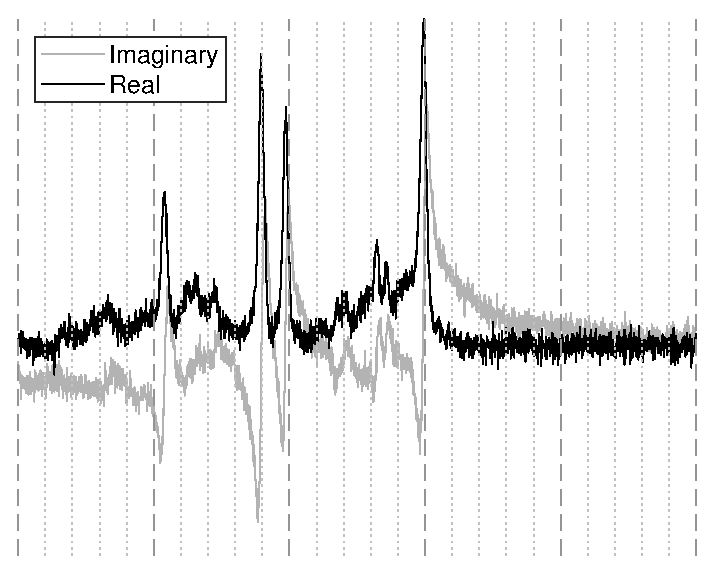
\includegraphics[width=0.95\textwidth,keepaspectratio]{images/phase/no_phase.eps}
        \caption{Spectrum with no phase offsets}
        \label{subfig:no phase}        
    \end{subfigure}
    \begin{subfigure}{0.32\textwidth}
        \centering
        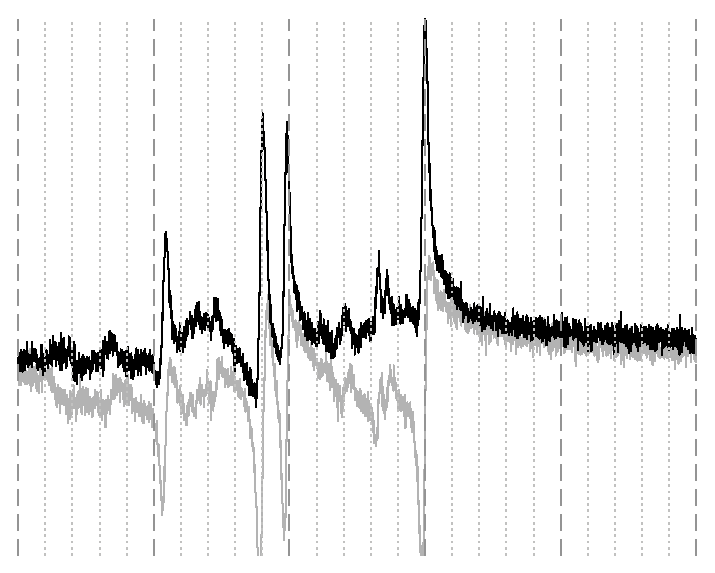
\includegraphics[width=0.95\textwidth,keepaspectratio]{images/phase/zero-order.eps}
        \caption{Spectrum with zero-order phase offset ($\phi_0 = 45^{\circ}$)}
        \label{subfig:zero order phase}        
    \end{subfigure}
    \begin{subfigure}{0.32\textwidth}
        \centering
        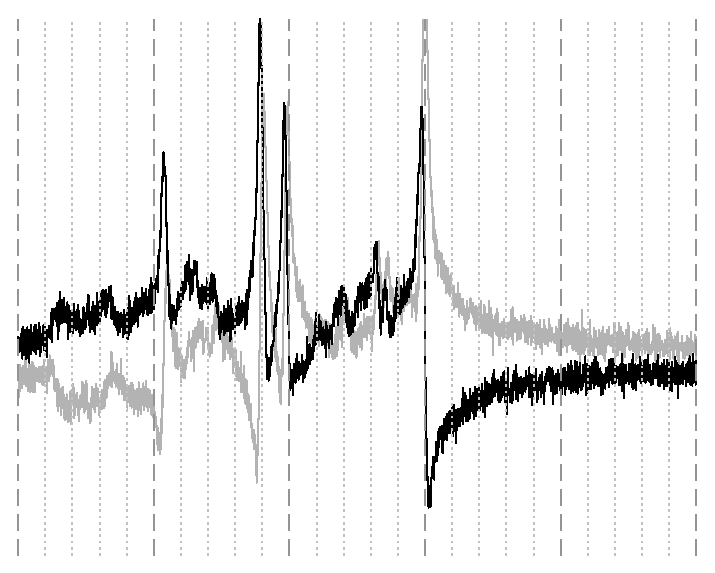
\includegraphics[width=0.95\textwidth,keepaspectratio]{images/phase/first-order.eps}
        \caption{Spectrum with first-order phase offset ($\phi_1 = 20^{\circ}$)}
        \label{subfig:first order phase}        
    \end{subfigure}
    \caption{These samples show how identical spectra are affected by zero- and first-order phase offsets. In \ref{subfig:no phase}, the real component (black) is in absorption mode exhibiting narrow line widths and is fully positive. In \ref{subfig:zero order phase}, a zero-order phase offset is applied. As the spectrum shifts from absorption to dispersion mode, the peaks uniformly lose their symmetry and negative values from the imaginary component are transferred to the real component. In \ref{subfig:first order phase}, a first-order phase shift is applied. This is evident because the asymmetry increases across the spectrum and emanates from the water peak.}
    \label{fig:phase effects}
\end{figure}
 
\subsubsection{Frequency Shifts}
% Frequency shifts observed in a spectrum result from complex interactions with a variety of factors. 
During data acquisition, the FID experiences a global frequency shift. However, some functional groups 
%individual moieties from metabolites and nuisance signals from macromolecules, lipids, and fats such as diglycerides and triglycerides, 
can experience individual frequency shifts which are attributed to effects such as temperature and pH. Similar to Sec. \ref{subsubsec:lineshapes}, the bare minimum requires separate global frequency shifts for the metabolites and nuisance signals. However, this model also allows each basis function to have an independent frequency shift in addition to the global shift which is in line with common spectral fitting protocols. For more in vivo-like, realistic spectra, values can be used from the work by Wermter \etal\cite{Wermter2017} which characterized the temperature-induced frequency shift of several brain metabolite moieties with temperature sensitivity. As more metabolites are characterized for their temperature- and pH-sensitivities, this information can be added to simulate more realistic spectra. Currently available data will be included in the table in the appendix.
 
\subsubsection{Eddy Currents}
% Eddy currents are common artifacts in MRI acquisitions that are induced by changes in the magnetic field, typically caused by the imaging gradients and present as time-dependent resonant frequency shifts. 
Eddy current correction techniques, such as the Klose\cite{Klose1990}, tend to be non-parameterized, making it difficult to model the exact effect of each approach. Near \etal\ in FID-A\cite{Simpson2017}, however, provide a parameterized equation for simulating first-order eddy currents. These artifacts are applied as a function of amplitude, $A$, time constant, $tc$, and time, $t$. The time constant must be short enough that it occurs entirely within the recorded echo, otherwise it will appear as a simple, global frequency shift. The effects of eddy currents can be seen in Fig. \ref{fig:eddy currents}.

\begin{figure}
    \centering
    % \begin{subfigure}{0.32\textwidth}
    %     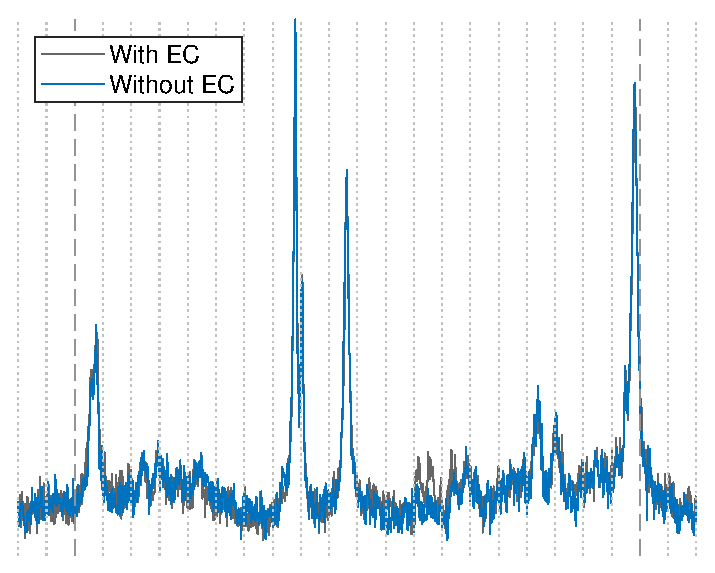
\includegraphics[width=0.95\textwidth, keepaspectratio]{images/eddy/ec=1.eps}
    %     \caption{Eddy current amplitude = 1.0}
    %     \label{subfig:ec=1}        
    % \end{subfigure}
    % \begin{subfigure}{0.32\textwidth}
    %     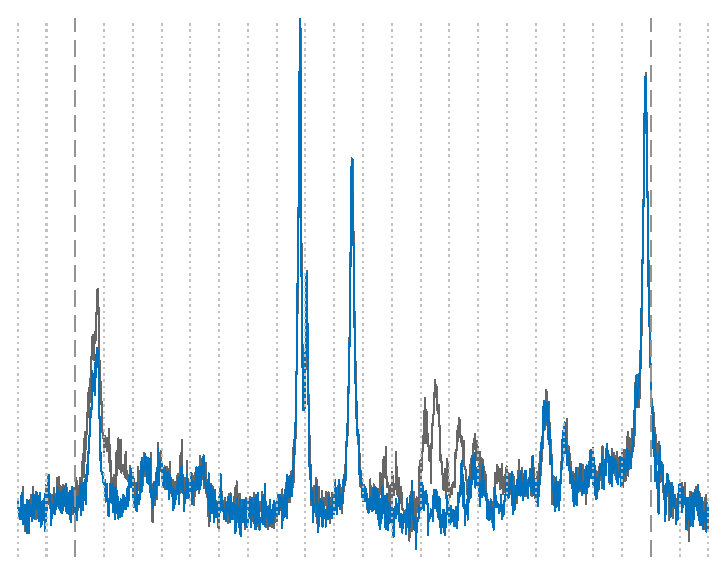
\includegraphics[width=0.95\textwidth, keepaspectratio]{images/eddy/ec=3.eps}
    %     \caption{Eddy current amplitude = 3.0}
    %     \label{subfig:ec=3}        
    % \end{subfigure}
    % \begin{subfigure}{0.32\textwidth}
    %     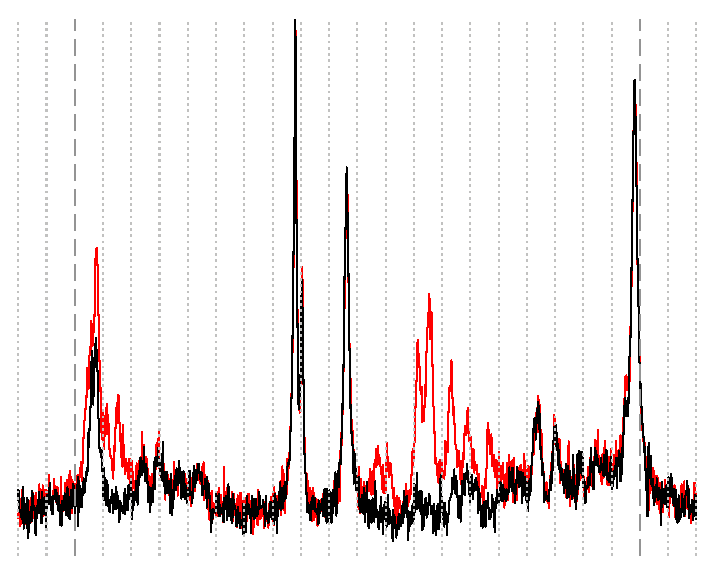
\includegraphics[width=0.95\textwidth, keepaspectratio]{images/eddy/ec=5.eps}
    %     \caption{Eddy current amplitude = 5.0}
    %     \label{subfig:ec=5}        
    % \end{subfigure}
    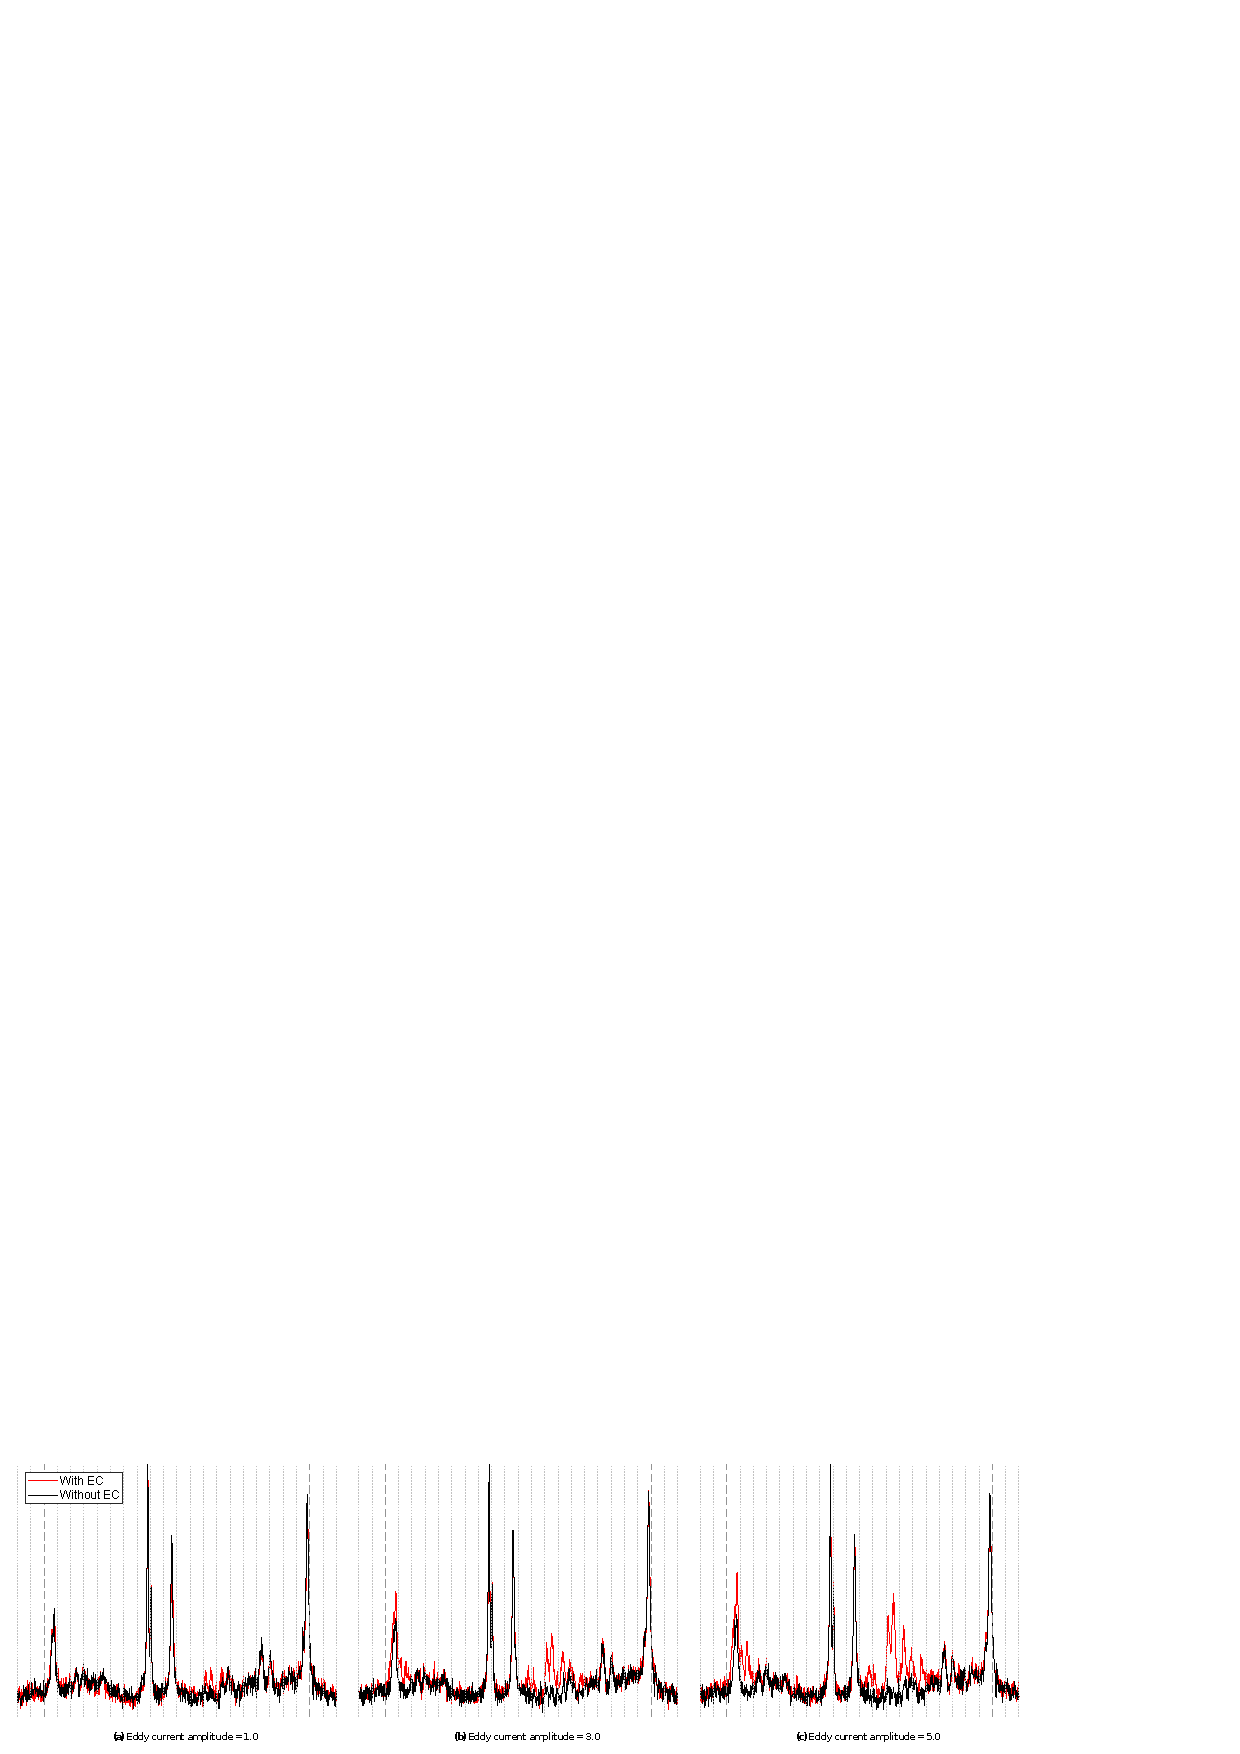
\includegraphics[width=\textwidth,keepaspectratio]{images/compiled_figures/MRS-Sim_Figure6_ eddy_current_effects.png}
    \caption{These 3 samples show the effect of eddy currents on MRS spectra to various degrees. The strength of the eddy currents increases from \ref{subfig:ec=1} to \ref{subfig:ec=5}. If the time constant, $tc$, is set too long, the eddy current artifact will appear as a global frequency shift. In these examples, it can be seen that only some frequencies are affected.}
    \label{fig:eddy currents}
\end{figure}


\subsubsection{Multi-Coil Transients}
When simulating transients, additional considerations need to be included. 
During acquisition, transients 
% A transient copy is made for each coil in the simulated scenario. These transients will 
experience additional artifacts including zero-order phase and frequency drifts, scaling due to coil sensitivity, and decreased SNR values. Each of these are included in the proposed framework. To allow for maximum variation in the simulations, each parameter can be sampled from distributions and is discussed below.

\paragraph{Noise} Averaging multi-coil acquisitions leads to an SNR improvement of the final spectrum by a factor of the square root of the number of non-zero weighted transients. To vary the SNR among the transients, this model scales the target linear SNR according to the number of coils and then samples scaling factors from a narrow normal distribution to maintain the mean target SNR. 

\paragraph{Frequency Drift and Phase Drift}
Frequency drifts and phase drifts are phenomena observed in multi-coil acquisitions in which each coil transient has an independent offset. %The lower SNR values of the transients make it harder to accurately correct these inter-transient variations. Therefore, drifts are typically minimized between the transients, called alignment. Proper alignment will preserve the underlying spectral features once the transients are combined.
These offsets and alignments are shown in Fig. \ref{fig:simulated transients}.

\begin{figure}[t]
    \centering
    \begin{subfigure}{0.32\textwidth}
        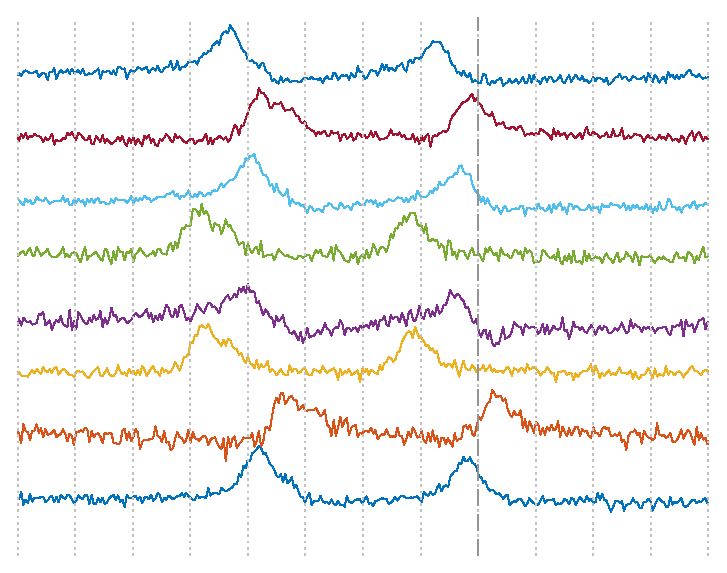
\includegraphics[width=0.95\textwidth, keepaspectratio]{images/samples_transients/8coil_w_phase_w_fshift_cropped.eps}
        \caption{Raw spectral transients}
        \label{subfig:raw transients}        
    \end{subfigure}
    \begin{subfigure}{0.32\textwidth}
        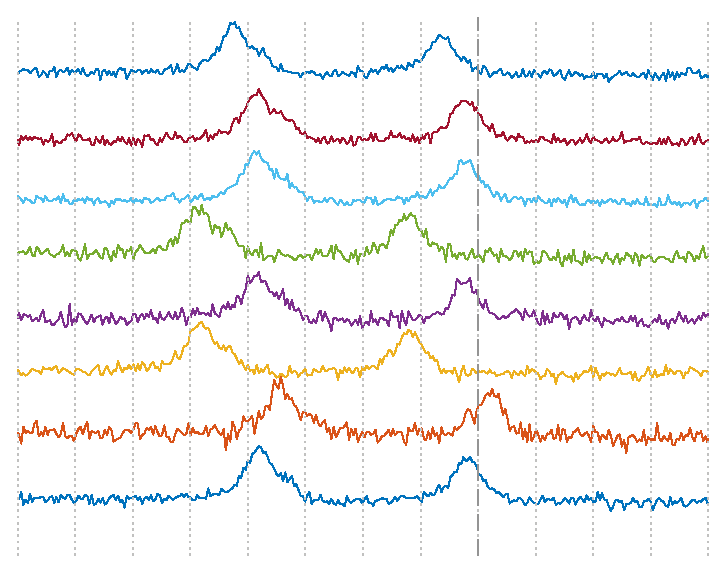
\includegraphics[width=0.95\textwidth, keepaspectratio]{images/samples_transients/8coil_wo_phase_w_fshift_cropped.eps}
        \caption{Phase alignment}
        \label{subfig:phase alignment}        
    \end{subfigure}
    \begin{subfigure}{0.32\textwidth}
        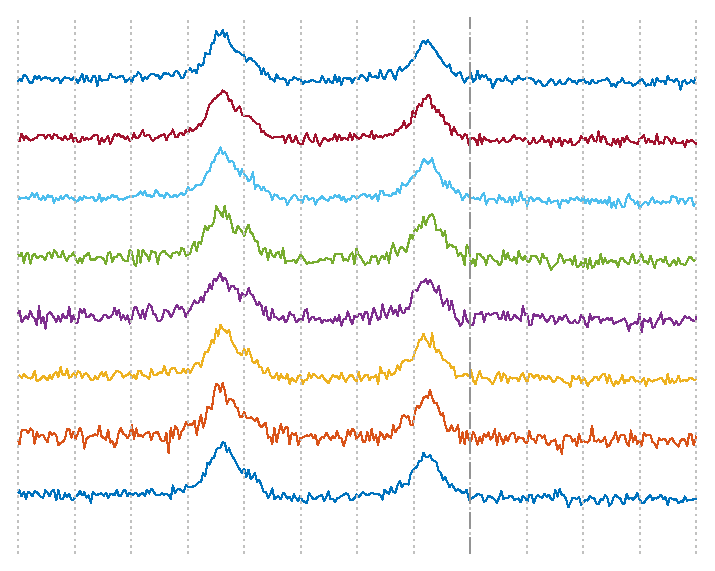
\includegraphics[width=0.95\textwidth, keepaspectratio]{images/samples_transients/8coil_wo_phase_wo_fshift_cropped.eps}
        \caption{Frequency alignment}
        \label{subfig:frequency alignment}        
    \end{subfigure}
    \caption{Examples of 8 simulated coil transients for a 3T GE PRESS sequence with TE=30ms. \ref{subfig:raw transients} shows transients with various SNRs and coil sensitivities along with zero-order phase and frequency offsets. \ref{subfig:phase alignment} shows the transients after phase alignment. \ref{subfig:frequency alignment} shows the transients after frequency alignment. After \ref{subfig:frequency alignment}, the transients can be averaged together and the coil-combined spectrum can then be fitted.}
    \label{fig:simulated transients}
\end{figure}

 
\paragraph{Coil Sensitivity}
A variety of coil combination techniques can be used to successfully combine multi-coil spectra. While these techniques differ in how they calculate the weights, all of them use weights to scale the transients before averaging. Assigning context, such as water peak height or coil sensitivity maps, to these weights when planning the simulations can help define the necessary parameter ranges and distributions to be in line with a given acquisition protocol.
 
\subsubsection{Final Steps} The desired use case will determine if a FID or a spectrum is necessary. If a FID is required, the simulation is finished and the data will be exported. If a spectrum is required, the Fourier transform will recover the spectrum at which point it can be cropped and resampled to a desired ppm range and spectral length. The default interpolation technique in this framework is a cubic Hermite modified Akima interpolator with momentum.


\subsection{Exporting Data}\label{subsec:exporting data}
The default export file format is .mat. These files include the data, spectral fits, simulation parameters, baseline offsets, and quantification results. To facilitate using the simulated spectra in various software packages, they are also exported in the NIfTI-MRS format\cite{Clarke2022}.
 
\subsection{Fitting Parameter Analysis}\label{subsec:Fitting Parameter Analysis}
The process of simulating a new dataset requires careful consideration of various factors, including the selection of appropriate parameter ranges and distributions. The optimal customization of these parameters depends on the intended use and application of the dataset. For instance, deep learning-based quantification models benefit from independent, uniform distributions that include all values the model will be expected to encounter. When validating a traditional spectral fitting model that includes soft constraints, it is crucial to incorporate those constraints when defining the parameter distributions. This ensures that the simulated dataset accurately reflects the underlying distribution of the target dataset. 

To mimic an in vivo dataset, accurate descriptions of clinical fitting parameters are crucially important. In collaboration with Osprey, it is now possible to export the spectral fitting parameters after quantification. Tools in this framework can then load the exported files and prepare the data for further analysis. Currently, this framework uses the python library Fitter\cite{Cokelaer2019} to identify the best fitting probability distribution for every parameter. \textit{A priori} knowledge, either from prior knowledge or data exploration, can narrow down the search range and speed up the analysis. The outputs for each parameter include evaluation metrics for the best performing distributions as well as a numerical characterization of the best fitting distribution.
 
\subsubsection{Recommendations}
The authors generally recommend that simulations include all relevant artifacts unless there is a specific reason to exclude them. A simulated dataset should include all phenomena that are expected to be encountered when the final work is deployed. Even highly accurate post-processing techniques have limitations and biases and leave some residue of the corrected artifacts. To ensure consistency between the simulated and clinical data, the artifacts should be included in the simulations and removed via the users’ own fitting protocols.  

Although not recommended, residual artifacts and post-processing techniques can be included in the simulations. Phase and frequency corrections can be simulated by applying a minimal offset during the initial simulation, which can be implemented in the parameter sampling protocol. Similarly, eddy currents can be scaled down by minimizing the sampled amplitudes. While not part of the acquisition protocol, apodization and zero filling are also possible. Apodization improves the SNR by multiplying the FID by a filter function, typically an exponential decay function or a Lorenztian-to-Gaussian transform. This framework implements an exponential decay as a function of time, $t$, and $T_L$ which defines the amount of apodization in Hz. Zero filling simply pads the FID with zeros to a defined length before the Fourier transform.

\subsection{Code}
This repository was written in PyTorch 1.11.0 and Python 3.9.7. Since this framework generates batches of spectra instead of individual spectra sequentially, a simulation batch size needs to be specified which will be affected by the spectral length and complexity of the simulations. As long as the batch size is set appropriately given the users' amount of RAM, this framework can be employed on standard computers without any special hardware. After publication, the repository will be available on GitHub, at \todo{https://www.github.com/REPOSITORY}, and MRSHub.

